\documentclass[11pt,a4paper,headsepline]{scrartcl}
\usepackage[utf8]{inputenc}
\usepackage[T1]{fontenc}
\usepackage[ngerman]{babel}
\usepackage{amsmath}
\usepackage{amsthm}
\usepackage{amssymb}
\usepackage{amsfonts}
\usepackage[scaled]{helvet}
\usepackage{amssymb}
\usepackage{multirow}
\usepackage{textcomp}
\usepackage{graphicx}
\usepackage{paralist}
\usepackage{textcomp}
\usepackage{pdflscape} 
\usepackage{marvosym}
\usepackage{float}
\usepackage{siunitx}
\usepackage[siunitx,european,cuteinductors,smartlabels]{circuitikz}
\usepackage{fancyhdr}
\usepackage{pgfplots}
\usepackage{sansmath}
\usetikzlibrary{shapes.geometric}
\usepackage{wasysym}
\usepackage[nix]{optional}
\usepackage{listings}
\lstset{
commentstyle=\color{green!50!black}}

\usetikzlibrary{calc}


%\theoremstyle{definition}
\newtheorem{aufgabe}{Aufgabe}
\newtheorem{loesung}{L\"osung}
\newcommand{\Var}{\operatorname{Var}}
\newcommand{\D}{\operatorname{d}}
\newcommand{\mum}{\operatorname{\mu m}}
\newcommand{\E}{\operatorname{E}}
\newcommand{\var}{\operatorname{var}}
\newcommand{\Id}{\operatorname{Id}}
\newcommand{\rg}{\operatorname{rg}}



\renewcommand*\familydefault{\sfdefault}
%\renewcommand{\arraystretch}{1.1}


\KOMAoptions{parskip=half,DIV=15,fontsize=11pt}
\unitlength1cm
\newif\ifuelsg %als slides
%\uelsgtrue
\uelsgfalse
\newif\ifnotuelsg
\ifuelsg\notuelsgfalse\else\notuelsgtrue\fi

\title{Praktikum ``Simulation im Zustandsraum''}
\date{}
\makeatletter
\let\Title\@title
\let\Author\@author
\makeatother
\pagestyle{fancy}
\fancyhead[L]{Prof. Dr. Raphael Pfaff}
\fancyhead[R]{85745: Energieeffiziente Antriebsregelung}
\fancyfoot[L]{Datei: \jobname}
\fancyfoot[R]{Datum: \today
\begin{picture}(0,0)(0,0)\put(.5,0){
\includegraphics[height=5cm]{fh_logo}}\end{picture}}


\begin{document}

\maketitle
\thispagestyle{fancy}
\vspace{-2cm}
% \hyphenation{Abwei-chungen}

\section*{Berechnung und Darstellung in Matlab/Scilab}
\begin{aufgabe}[\"Uberf\"uhrung \"Ubertragungsfunktion in Zustandsraum]
\label{Task:Calc}
Nutzen Sie Matlab oder Scilab, um die \"Ubertragungsfunktion \[G(s) = \frac{3+s}{10+1.1s+s^{2}}\]  in eine Zustandsraumdarstellung zu \"uberf\"uhren.
Nutzen Sie (jeweils in Scilab):
\begin{itemize}
	\item \texttt{syslin}, um die \"Ubertragungsfunktion zu definieren,
	\item \texttt{tf2ss} zur \"Uberf\"uhrung in den Zustandsraum und 
	\item \texttt{csim}, um eine Sprungantwort des Systems aufzuzeichnen und mit \texttt{plot2d} zu plotten. 
\end{itemize}
\end{aufgabe}
\vspace{0.5cm}

\begin{aufgabe}[Steuerbarkeit und Beobachtbarkeit]
\label{Task:ContObs}
Bestimmen Sie die Steuerbarkeits- und Beobachtbarkeitsmatrizen und ihre R\"ange. Beurteilen Sie die Steuerbarkeit und Beobachtbarkeit.
\end{aufgabe}
\vspace{0.5cm}
\begin{aufgabe}[Phasendiagramm]
\label{Task:Phase}
Zeichnen Sie ein Richtungsfeld mit
\begin{equation*}
\begin{pmatrix}
 \dot{x}_{1} \\  \dot{x}_{2}
\end{pmatrix} = A 
\begin{pmatrix}
 {x}_{1} \\  {x}_{2}
\end{pmatrix}
\end{equation*}
als Richtung eines Pfeils an der Koordinate $\left(x_{1}, x_{2} \right)$. W\"ahlen Sie den Bereich $x_{1,2} = -1 \ldots 1$.

Welche Bedeutung hat dieses Richtungsfeld? Welche Eigenschaften des Systems lassen sich ablesen?

Hinweise:
\begin{itemize}
	\item Definieren Sie eine Funktion \texttt{xdot}, um die Richtung der Pfeile zu bestimmen.
	\item Definieren Sie eine globale Variable zur Speicherung der Systemmatrix.
	\item Nutzen Sie die Funktion  \texttt{quiver} (Matlab) bzw. \texttt{fchamp} (Scilab), um ein Richtungsfeld zu plotten.
	\item Optional: Erg\"anzen Sie eine Trajektorie des System im Richtungsfeld.
\end{itemize}
\end{aufgabe}

\opt{loesung}{
\newpage
\begin{loesung}[Skript zur L\"osung der Aufgaben \ref{Task:Calc}, \ref{Task:ContObs} und  \ref{Task:Phase}] $ $ \\
\lstinputlisting[language=Scilab]{../Loesungen/151203P113.sce}

\begin{figure}[htbp]
\begin{center}
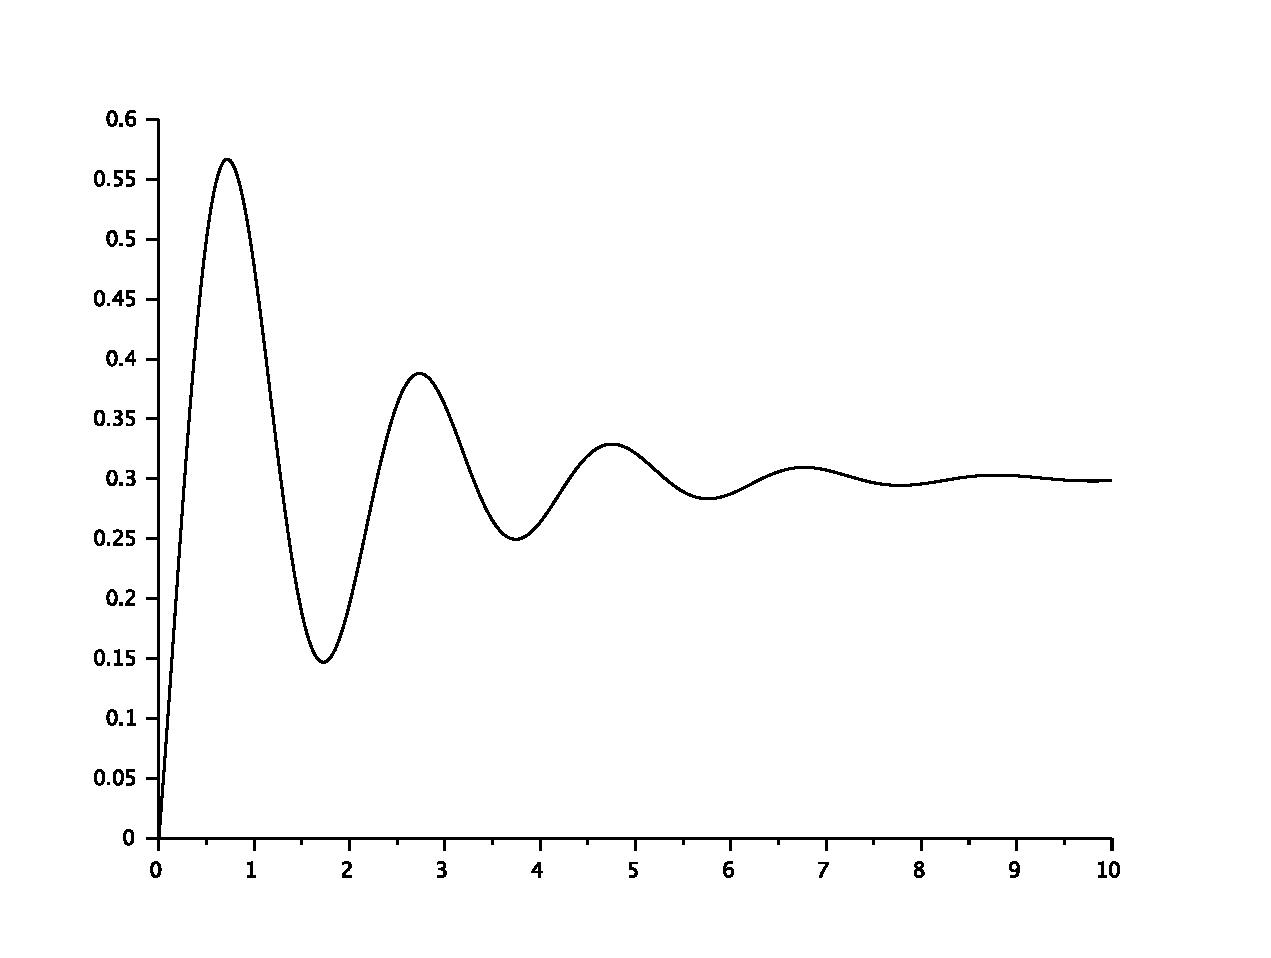
\includegraphics[width = 0.6\textwidth]{Sprung}
\caption{Ausgabe der Sprungantwort}
\label{default}
\end{center}
\end{figure}

\begin{figure}[htbp]
\begin{center}
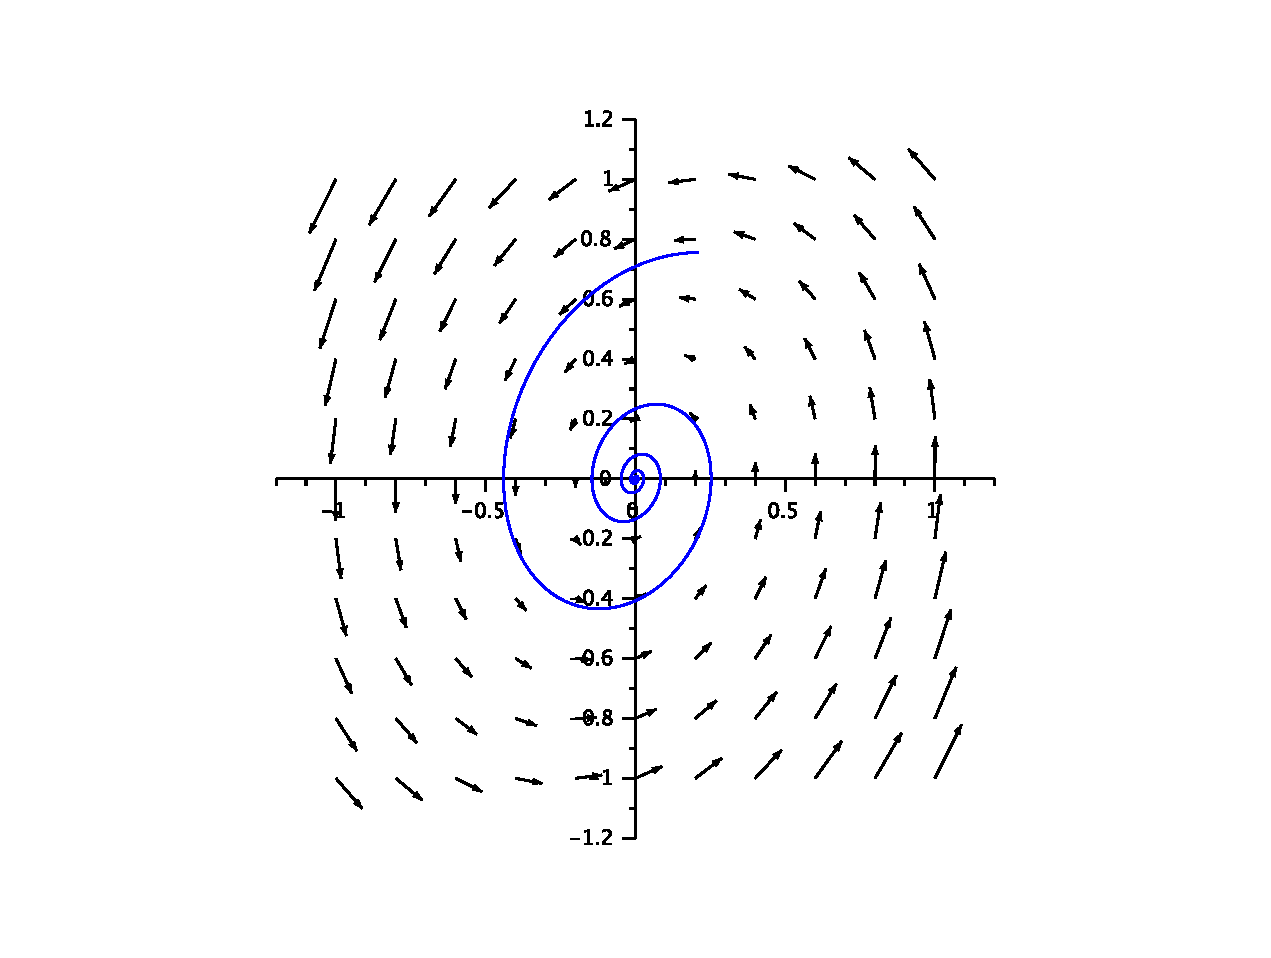
\includegraphics[width = 0.6\textwidth]{Trajektorie}
\caption{Ausgabe des Richtungsfeldes und der Trajektorie}
\label{default}
\end{center}
\end{figure}

\end{loesung}
}

\section*{Simulation in Scicos}
\begin{aufgabe}[Erstellen eines Blockdiagramms in Scicos] 
\label{Task:BDScicos}
Erstellen Sie ein Blockdiagramm eines Systems in Regelungsnormalform mit folgender Systembeschreibung
\begin{equation*}
		\frac{\D^{n} y}{\D t^{n}} + a_{1} \frac{\D y}{\D t} + a_{0} y  
		= b_{0} u 
	\end{equation*}
	und den Parametern $a_{0} = 1$, $a_{1} = 0{,}2$ und $b_{0} = 1$.
	
	\begin{enumerate}[a)]
		\item Die Eingangsgr\"o{\ss}e in das System sei ein Sprung bei $t = 0$.
		\item Nutzen Sie eine geeignete Senke, um die Antwort des Systems beobachten zu k\"onnen.
	\end{enumerate}
\end{aufgabe}
\vspace{0.5cm}
\begin{aufgabe}[Ausf\"uhrung mittels Scilab]
\label{Task:Scilab}
Modifizieren Sie das Blockdiagramm aus Aufgabe \ref{Task:BDScicos} so, dass Sie
\begin{itemize}
		\item die Systemparameter und
		\item die Eingangsgr\"o{\ss}e
		\end{itemize}
in Scilab definieren k\"onnen. 

Erstellen Sie in Programm in Scilab, das es Ihnen erm\"oglicht
\begin{itemize}
		\item die Parameter und Eingangsgr\"o{\ss}e zu definieren,
		\item das Blockdiagramm auszuf\"uhren und
		\item Eingangsgr\"o{\ss}e und Zustandsgr\"o{\ss}en in einen gemeinsamen Diagramm darzustellen.
		\end{itemize}
\end{aufgabe}
\opt{loesung}{
\newpage
\begin{loesung}[Skript zur L\"osung der Aufgaben \ref{Task:Scilab}] $ $ \\
\lstinputlisting[language=Scilab]{../Loesungen/151202P145.sce}

\begin{figure}[htbp]
\begin{center}
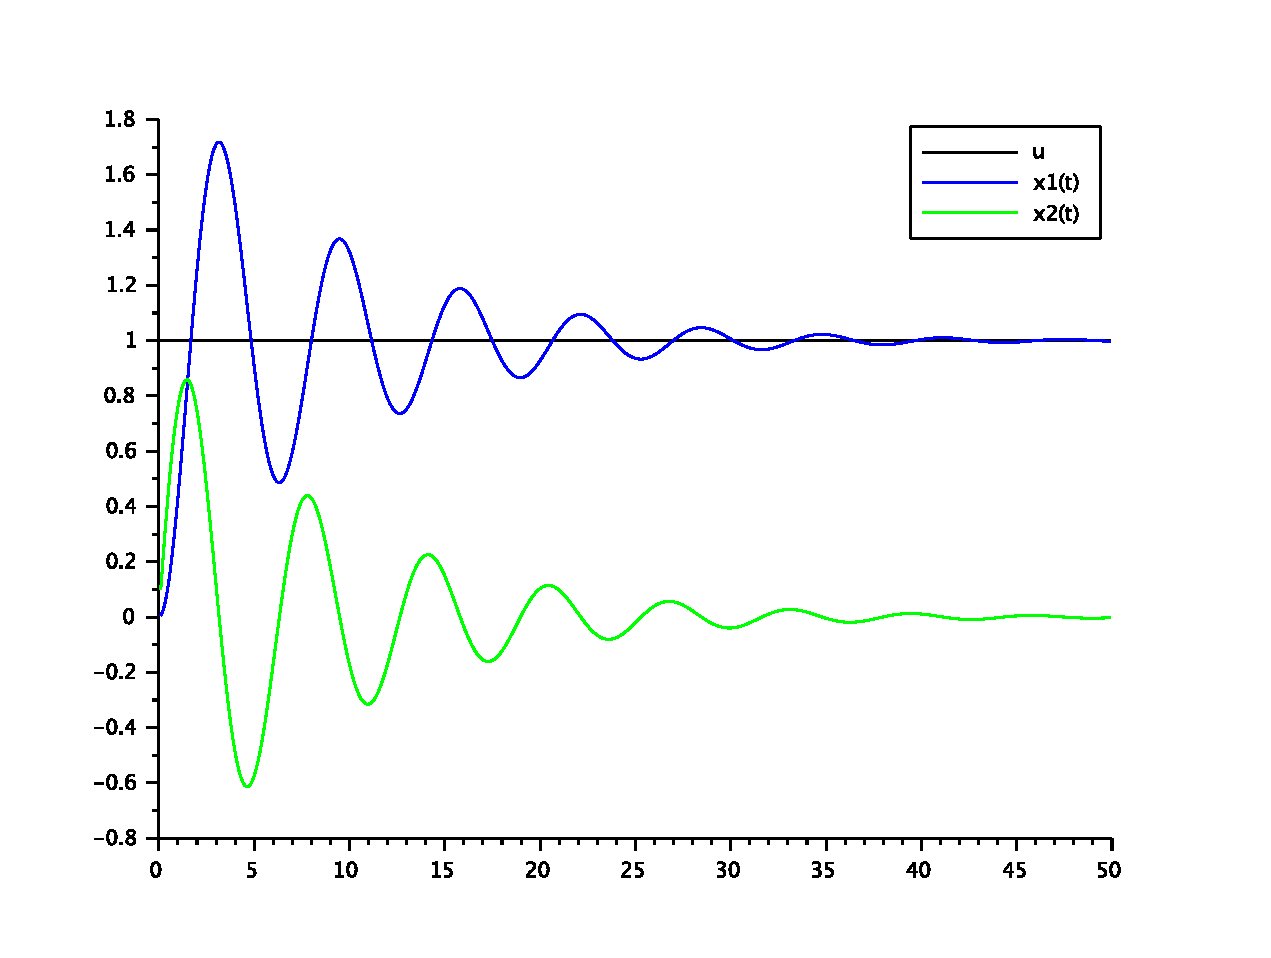
\includegraphics[width = 0.6\textwidth]{P1Output}
\caption{Ausgabe der Sprungantwort}
\label{default}
\end{center}
\end{figure}
\end{loesung}
}

\end{document}